\documentclass[11pt,a4paper]{article}

\usepackage[utf8]{inputenc}
\usepackage[T1]{fontenc}
\usepackage{lmodern}
\usepackage{microtype}
\usepackage[margin=1in]{geometry}
\usepackage{amsmath,amssymb,amsthm}
\usepackage{mathtools}
\usepackage{bm}
\usepackage{graphicx}
\usepackage{booktabs}
\usepackage{array}
\usepackage{xcolor}
\usepackage{hyperref}
\usepackage{cleveref}
\usepackage{listings}
\usepackage{caption}
\usepackage{tikz}
\usetikzlibrary{arrows.meta, positioning}
\usepackage{natbib}
\usepackage{authblk}
\usepackage{enumitem}
\usepackage{tcolorbox}
\tcbuselibrary{breakable, skins}

\hypersetup{
  colorlinks=true,
  linkcolor=blue!70!black,
  citecolor=green!50!black,
  urlcolor=blue!70!black,
  pdftitle={LOGOS: A Physics-Informed Language Model in C++/CUDA},
  pdfauthor={LOGOS Research Team},
  pdfkeywords={LLM, Physics-Informed, CUDA, Transformer, Hamiltonian Mechanics, Navier-Stokes}
}

\newcommand{\LOGOS}{\textsc{LOGOS}}
\newcommand{\calF}{\mathcal{F}}
\newcommand{\calH}{\mathcal{H}}
\newcommand{\calL}{\mathcal{L}}
\newcommand{\btheta}{\bm{\theta}}
\newcommand{\CE}{\mathrm{CE}}
\newcommand{\softmax}{\mathrm{softmax}}

\lstset{
  language=C++,
  basicstyle=\ttfamily\footnotesize,
  keywordstyle=\color{blue!80!black}\bfseries,
  numbers=left,
  numberstyle=\tiny\color{gray},
  numbersep=5pt,
  breaklines=true,
  frame=single,
  rulecolor=\color{gray!30},
  backgroundcolor=\color{gray!5},
  captionpos=b
}

\title{%
  \textbf{LOGOS: A Physics-Informed Language Model\\
  Implemented from Scratch in C++/CUDA}
}

\author[1]{LOGOS Research Team}
\affil[1]{Independent Research, Open Source Project}

\date{November 2026}

\begin{document}

\maketitle

\begin{abstract}
We describe \LOGOS{}, a decoder-only Transformer language model with
roughly 219 million parameters, trained on a bilingual Hindi--English
Wikipedia corpus, whose training and inference stack is written entirely
in C++20 and CUDA without an automatic-differentiation framework.
\LOGOS{} replaces several standard components with physics-motivated
alternatives: a hybrid Hamiltonian--Langevin optimiser, a Helmholtz
free-energy loss $\calF = \CE - T\cdot S$, Navier--Stokes-style advection
and diffusion applied to queries and values, a Reynolds-number-adaptive
layer normalisation, a Poincar\'e-ball token embedding, Feynman
$\beta$-dropout, and a path-integral learning-rate multiplier. All
matrix products use cuBLAS and attention uses a custom causal
Flash-Attention kernel. This report documents the design, the equations
implemented, the memory budget, and the training configuration. It does
\emph{not} report benchmark results: training runs so far are partial,
and controlled ablations against AdamW and plain cross-entropy have not
been completed. We therefore present the components as design hypotheses
to be tested rather than as demonstrated improvements.
\end{abstract}

\textbf{Keywords:} Physics-Informed LLM, CUDA, Transformer, Hamiltonian
Mechanics, Navier--Stokes Attention, Free Energy Loss, Bilingual NLP.

\vspace{1em}
\hrule
\vspace{1em}

\section{Introduction}
\label{sec:intro}

Most large language models share one recipe: full self-attention, the
AdamW optimiser, and a cross-entropy loss~\citep{brown2020gpt3,chowdhery2022palm,touvron2023llama}.
\LOGOS{} is a research codebase for testing alternatives to three parts
of that recipe, and for doing so in a stack small enough to read end to
end.

\begin{enumerate}[label=(\roman*)]
  \item \textbf{Optimisation.}
    Hybrid Hamiltonian--Langevin dynamics~\citep{neal2011mcmc,ma2015complete}
    are well studied for Bayesian inference but are rarely used as the
    primary optimiser of a Transformer.
  \item \textbf{Attention.}
    Softmax attention is a Boltzmann weighting over positions~\citep{ramsauer2020hopfield}.
    We test whether adding explicit transport terms (advection of queries,
    viscous diffusion of values) is useful.
  \item \textbf{Loss.}
    Cross-entropy ignores the entropy of the output distribution. A
    Helmholtz free-energy objective $\calF = U - TS$ adds a
    temperature-weighted entropy term.
\end{enumerate}

\begin{tcolorbox}[colback=blue!3, colframe=blue!40!black,
                  title=\textbf{Contributions}, breakable]
\begin{enumerate}
  \item \textbf{SHM Optimizer}: hybrid Hamiltonian--Langevin update with
        a cosine-annealed mixing coefficient (\S\ref{sec:shm}).
  \item \textbf{Free Energy Loss}: $\calF = \CE - T\cdot S$ with
        temperature annealing and an analytic entropy gradient
        (\S\ref{sec:free_energy}).
  \item \textbf{Navier--Stokes Attention}: advection on queries and
        diffusion on values, blended with standard attention
        (\S\ref{sec:ns_attn}).
  \item \textbf{Reynolds LayerNorm}: normalisation scale modulated by a
        turbulence-style Reynolds number (\S\ref{sec:reynolds}).
  \item \textbf{Causal Flash Attention kernel}: tiled online-softmax
        attention with $\mathcal{O}(\text{seq}\cdot d_h)$ memory
        (\S\ref{sec:flash}).
  \item \textbf{Hyperbolic embedding}: Poincar\'e-ball embedding via
        $\exp_0$ with an analytic Jacobian backward pass
        (\S\ref{sec:hyperbolic}).
  \item \textbf{Feynman $\beta$-Dropout} and \textbf{Path-Integral LR}
        (\S\ref{sec:feynman_dropout}, \S\ref{sec:path_integral}).
  \item A hand-written forward/backward implementation on cuBLAS with
        checkpoint-resume training (\S\ref{sec:impl}).
\end{enumerate}
\end{tcolorbox}

\section{Background and Related Work}
\label{sec:related}

\paragraph{Physics-informed networks.}
Physics-informed neural networks~\citep{raissi2019pinns} add physical
constraints to the loss. \LOGOS{} instead changes operations inside the
network and the training dynamics.

\paragraph{Hamiltonian Monte Carlo and Langevin dynamics.}
HMC~\citep{duane1987hybrid,neal2011mcmc} uses symplectic leapfrog
integration; stochastic gradient Langevin dynamics~\citep{welling2011bayesian}
injects temperature-scaled Gaussian noise into gradient steps. The SHM
optimiser interpolates between the two with a coefficient
$\alpha_H\in[0,1]$.

\paragraph{Efficient attention.}
FlashAttention~\citep{dao2022flashattention} avoids materialising the
$\text{seq}\times\text{seq}$ score matrix by tiling through on-chip
memory. \LOGOS{} implements a causal version of this algorithm directly
in CUDA.

\paragraph{Hyperbolic representations.}
Poincar\'e embeddings~\citep{nickel2017poincare} represent hierarchical
structure compactly. \LOGOS{} uses the exponential map at the origin as
the token-embedding layer of a generative model.

\section{Model Architecture}
\label{sec:arch}

\LOGOS{} is a decoder-only Transformer.

\begin{table}[htbp]
\centering
\caption{Production configuration.}
\label{tab:arch}
\begin{tabular}{lll}
\toprule
\textbf{Symbol} & \textbf{Value} & \textbf{Description}\\
\midrule
$d$             & 1024           & Model dimension\\
$L$             & 16             & Transformer blocks\\
$H$             & 16             & Attention heads per block\\
$d_h$           & 64             & Head dimension ($d/H$)\\
$T_{\max}$      & 8192           & Maximum sequence length\\
$V$             & 8192           & BPE vocabulary size\\
$N_{\text{param}}$ & $\approx$219M & Trainable parameters\\
\bottomrule
\end{tabular}
\end{table}

The forward pass is
\begin{align}
  \mathbf{E} &= \exp_0(\mathbf{W}_e \cdot \mathbf{x})
               \quad\text{(hyperbolic embedding)}\\
  \mathbf{H}^{(0)} &= \mathbf{E} + \mathbf{PE}\\
  \mathbf{H}^{(\ell)} &= \mathbf{H}^{(\ell-1)}
    + \mathrm{NS}\text{-}\mathrm{MHA}\!\left(\mathrm{ReLN}\!\left(\mathbf{H}^{(\ell-1)}\right)\right)
    + \mathrm{FFN}_{\text{Feynman}}\!\left(\mathrm{ReLN}\!\left(\mathbf{H}^{(\ell-1)}\right)\right)\\
  \hat{\mathbf{y}} &= \mathbf{H}^{(L)}\,\mathbf{W}_{\text{lm}}
    \quad\text{(cuBLAS GEMM)}\\
  \mathcal{L} &= \calF\!\left(\hat{\mathbf{y}},\;y;\;T\right)
\end{align}
where $\mathbf{PE}$ is a learned position embedding, $\mathrm{ReLN}$ is
Reynolds layer normalisation, and $\mathrm{NS}\text{-}\mathrm{MHA}$ is
multi-head attention with Navier--Stokes terms.

\begin{figure}[htbp]
\centering
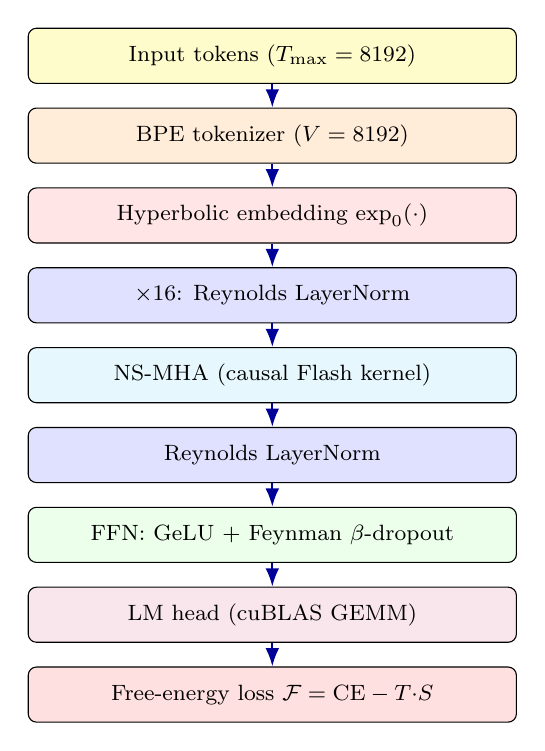
\begin{tikzpicture}[
  box/.style={rectangle, draw, rounded corners=3pt,
              minimum width=6.2cm, minimum height=0.7cm,
              text centered, font=\footnotesize},
  arrow/.style={-Latex, thick, color=blue!60!black}
]
\node[box, fill=yellow!20] (input) {Input tokens ($T_{\max}=8192$)};
\node[box, fill=orange!15, below=0.3cm of input] (bpe) {BPE tokenizer ($V=8192$)};
\node[box, fill=red!10, below=0.3cm of bpe] (hyp) {Hyperbolic embedding $\exp_0(\cdot)$};
\node[box, fill=blue!12, below=0.3cm of hyp] (ln1) {$\times 16$: Reynolds LayerNorm};
\node[box, fill=cyan!10, below=0.3cm of ln1] (mha) {NS-MHA (causal Flash kernel)};
\node[box, fill=blue!12, below=0.3cm of mha] (ln2) {Reynolds LayerNorm};
\node[box, fill=green!8, below=0.3cm of ln2] (ffn) {FFN: GeLU + Feynman $\beta$-dropout};
\node[box, fill=purple!10, below=0.3cm of ffn] (lmh) {LM head (cuBLAS GEMM)};
\node[box, fill=red!12, below=0.3cm of lmh] (loss) {Free-energy loss $\calF=\CE-T{\cdot}S$};
\foreach \from/\to in {input/bpe, bpe/hyp, hyp/ln1, ln1/mha, mha/ln2, ln2/ffn, ffn/lmh, lmh/loss}
  \draw[arrow] (\from) -- (\to);
\end{tikzpicture}
\caption{End-to-end architecture.}
\label{fig:arch}
\end{figure}

\section{Components}
\label{sec:physics}

\subsection{SHM Optimizer: Stochastic Hamiltonian Mechanics}
\label{sec:shm}

Treat the parameter vector $\btheta$ as position and the velocity
$\mathbf{v}$ as momentum, with
\begin{equation}
  \calH(\btheta, \mathbf{v}) = \calL(\btheta) + \tfrac{1}{2}\mathbf{v}^\top\mathbf{v}.
\end{equation}
Symplectic leapfrog integration with step $\epsilon$ is
\begin{align}
  \mathbf{v}_{t+\frac{1}{2}} &= \mathbf{v}_t - \frac{\epsilon}{2}\nabla_\theta \calL(\btheta_t)\\
  \btheta_{t+1} &= \btheta_t + \epsilon\,\mathbf{v}_{t+\frac{1}{2}}\\
  \mathbf{v}_{t+1} &= \mathbf{v}_{t+\frac{1}{2}} - \frac{\epsilon}{2}\nabla_\theta \calL(\btheta_{t+1}).
\end{align}
The Langevin component adds temperature-scaled noise,
\begin{equation}
  \btheta_{t+1} = \btheta_t - \frac{\epsilon}{2}\nabla_\theta\calL + \sqrt{\epsilon\,T}\,\bm{\xi}_t,
  \quad \bm{\xi}_t \sim \mathcal{N}(\mathbf{0}, \mathbf{I}).
\end{equation}
The hybrid update mixes the two:
\begin{equation}
  \mathbf{v}_{t+\frac{1}{2}} = \mu\,\mathbf{v}_t
    - \alpha_H(t)\tfrac{\epsilon}{2}\nabla_\theta\calL
    - \alpha_L(t)\tfrac{\epsilon}{2}\gamma\mathbf{v}_t
    + \sqrt{\gamma\,T(t)\,\epsilon\,\alpha_L(t)}\,\bm{\xi}_t,
\end{equation}
with $\alpha_H(t)+\alpha_L(t)=1$, friction $\gamma$, and the annealed
temperature
\begin{equation}
  T(t) = \max\!\left(T_{\min},\;
         T_{\text{end}} + (T_{\text{start}}-T_{\text{end}})
         \cdot\tfrac{1+\cos(\pi t/t_{\max})}{2}\right),
  \qquad T_{\min}=10^{-3}.
\end{equation}
$\alpha_H$ is cosine-annealed from a Langevin-dominant value
($0.3$) to a Hamiltonian-dominant value ($0.99$) over training. The
update runs as a single fused CUDA kernel over the flat parameter and
velocity buffers.

\subsection{Free Energy Loss}
\label{sec:free_energy}

With $p=\softmax(\hat{\mathbf{y}})$ and Shannon entropy
$S=-\sum_v p_v\log p_v$, the loss is
\begin{equation}
  \calF(\hat{\mathbf{y}}, y;\,T) = -\log p_y \;-\; T\,S.
\end{equation}
The gradient with respect to logit $\hat{y}_v$ is
\begin{equation}
  \frac{\partial\calF}{\partial \hat{y}_v}
  = (p_v - \mathbf{1}[v=y]) + T\,p_v\!\left(\log p_v + S\right).
\end{equation}
Minimising $\calF$ rewards higher output entropy, so the extra term acts
as a regulariser against over-confident predictions. $T$ is
cosine-annealed from $1.0$ to a floor of $10^{-3}$, so the loss
approaches plain cross-entropy late in training. The effect is similar in
spirit to label smoothing with a decaying coefficient; whether it
improves generalisation here is an open question
(\S\ref{sec:status}).

\subsection{Navier--Stokes Attention}
\label{sec:ns_attn}

Standard attention computes
$\softmax(\mathbf{Q}\mathbf{K}^\top/\sqrt{d_h})\mathbf{V}$~\citep{vaswani2017attention}.
Viewing the sequence as a one-dimensional discretised velocity field,
the incompressible momentum equation is
\begin{equation}
  \frac{\partial\mathbf{u}}{\partial t}
  + (\mathbf{u}\cdot\nabla)\mathbf{u}
  = -\nabla p + \nu\nabla^2\mathbf{u}.
\end{equation}
\LOGOS{} applies an upwind advection step to queries and a
diffusion step to values:
\begin{align}
  \mathbf{Q}_{\text{adv}}[i] &= \mathbf{Q}[i] + \eta\,(\mathbf{Q}[i] - \mathbf{Q}[i-1]),
  \qquad \eta=0.1,\\
  \mathbf{V}_{\text{smooth}}[i] &= (1-\nu)\,\mathbf{V}[i]
    + \tfrac{\nu}{2}\,(\mathbf{V}[i-1]+\mathbf{V}[i+1]),
  \qquad \nu=0.05.
\end{align}
The output blends the standard and Navier--Stokes paths,
\begin{equation}
  \mathbf{out} = (1-\alpha)\,\mathrm{Attn}_{\text{std}} + \alpha\,\mathrm{Attn}_{\text{NS}},
  \qquad \alpha=0.3.
\end{equation}
This is an analogy, not a derivation: the softmax rows sum to one, but
no claim is made that the scheme solves the Navier--Stokes equations.

\subsection{Reynolds LayerNorm}
\label{sec:reynolds}

Standard layer normalisation is
$\gamma\odot(\mathbf{h}-\mu)/(\sigma+\epsilon)+\beta$.
Reynolds LayerNorm modulates $\gamma$ using
\begin{equation}
  \mathrm{Re}(\mathbf{h}) = \frac{\|\mathbf{h}\|_2\,\mu}{\sigma + \epsilon},
  \qquad
  \gamma_{\mathrm{Re}} = \frac{\gamma}{1 + \mathrm{Re}/\mathrm{Re}_{\text{ref}}},
\end{equation}
so high-variance (``turbulent'') activations are scaled down. The layer
keeps running mean and variance statistics, which are stored in
checkpoints and used at inference.

\subsection{Causal Flash Attention Kernel}
\label{sec:flash}

Materialising the score matrix costs $\mathcal{O}(\text{seq}^2)$ memory:
at $\text{seq}=8192$ and FP32 that is 268~MB per head. The kernel
streams $\mathbf{Q},\mathbf{K},\mathbf{V}$ in tiles and maintains running
softmax statistics $(\ell,m)$:
\begin{align}
  m_{\text{new}} &= \max(m_{\text{old}},\;\max_j s_{ij})\\
  \ell_{\text{new}} &= e^{m_{\text{old}}-m_{\text{new}}}\ell_{\text{old}} + \sum_j e^{s_{ij}-m_{\text{new}}}\\
  \mathbf{o}_{\text{new}} &= \frac{e^{m_{\text{old}}-m_{\text{new}}}\ell_{\text{old}}\,\mathbf{o}_{\text{old}} + \sum_j e^{s_{ij}-m_{\text{new}}}\mathbf{V}_j}{\ell_{\text{new}}}.
\end{align}
Memory is $\mathcal{O}(\text{seq}\cdot d_h)$. Attention is dense and
causal in both forward and backward passes. Earlier prototypes
explored a sparse window-plus-stride mask and an INT8 key--value cache;
neither was connected to the GPU training path, and both have been
removed.

\subsection{Hyperbolic Embedding}
\label{sec:hyperbolic}

Token embeddings are mapped into the Poincar\'e ball by
\begin{equation}
  \exp_0(\mathbf{v}) = \tanh(\|\mathbf{v}\|)\,\frac{\mathbf{v}}{\|\mathbf{v}\|}.
\end{equation}
The backward pass uses the analytic Jacobian
\begin{equation}
  \frac{\partial \exp_0(\mathbf{v})}{\partial \mathbf{v}}
  = \frac{\text{sech}^2(\|\mathbf{v}\|)}{\|\mathbf{v}\|}\mathbf{I}
  + \left(\frac{\tanh(\|\mathbf{v}\|)}{\|\mathbf{v}\|}
    - \frac{\text{sech}^2(\|\mathbf{v}\|)}{\|\mathbf{v}\|}\right)
    \frac{\mathbf{v}\mathbf{v}^\top}{\|\mathbf{v}\|^2},
\end{equation}
with a numerical floor of $10^{-8}$ on $\|\mathbf{v}\|$.

\subsection{Feynman \texorpdfstring{$\beta$}{beta}-Dropout}
\label{sec:feynman_dropout}

Retained activations are scaled by an amplitude factor $\beta\in(0,1]$:
\begin{equation}
  h_{\text{out},i} = \begin{cases}
    \beta \cdot h_i / p_{\text{keep}} & \text{if } u_i > p_{\text{drop}}\\
    0 & \text{otherwise}
  \end{cases}
  \qquad u_i\sim\mathcal{U}(0,1).
\end{equation}
The backward pass reuses the stored mask and applies the same factor.

\subsection{Path-Integral Learning Rate}
\label{sec:path_integral}

Using the weight trajectory as a path and a Wick-rotated amplitude, a
log-amplitude is accumulated:
\begin{equation}
  \log A_t = -\sum_{\tau=0}^{t} \frac{\calL(\btheta_\tau)\,\|\Delta\btheta_\tau\|}{\hbar},
\end{equation}
where $\hbar$ is a hyperparameter. The relative amplitude scales the
learning rate:
\begin{equation}
  \text{lr}(t) = \text{lr}_{\text{base}}\cdot
  \left[\eta_{\min} + (1-\eta_{\min})\cdot\frac{A_t}{A_{\text{best}}}\right].
\end{equation}
For efficiency an EMA variant is used,
$\text{EMA}_t = 0.98\,\text{EMA}_{t-1} + 0.02\,a_t$ with
$a_t=\calL_t\|\Delta\btheta_t\|$, scaling the learning rate by
$e^{-(a_t-\text{EMA}_t)/(\text{EMA}_t+\epsilon)}$.

\section{Implementation}
\label{sec:impl}

\paragraph{GEMM.}
Every forward and backward matrix product, including the LM head, goes
through cuBLAS via a single row-major wrapper. TF32 tensor-core math is
available as a build option on Ampere and newer GPUs.

\paragraph{Autograd.}
Backward passes are written by hand for every component. This is
necessary for the Feynman mask chain, the hyperbolic Jacobian, and the
entropy gradient of the free-energy loss, and it avoids graph
bookkeeping overhead.

\paragraph{Mixed precision.}
A manual AMP scheme keeps FP32 master weights with an FP16 shadow copy
and a dynamic loss scaler.

\paragraph{Host and device weights.}
A host-side weight container is used only for checkpoint I/O. The
checkpoint stores the embedding, LM head, learned position embedding,
all block weights, and the Reynolds running statistics, and training
resumes from it together with loader and optimiser state.

\paragraph{Multi-GPU.}
Data-parallel training on two GPUs is supported: micro-batches are split
between devices, gradients are reduced through the host, the optimiser
step runs on GPU~0, and updated weights are copied to GPU~1.

\section{Training Setup}
\label{sec:training}

\subsection{Dataset and Tokeniser}
Training data is about 1.5~GB of Wikipedia text (Hindi and English,
November 2023 dumps), cleaned and streamed by a prefetching
\texttt{StreamingDataLoader} with 4--64~MB chunks depending on GPU tier.
A byte-pair-encoding tokeniser with $V=8192$ is trained from scratch on
the combined corpus, covering Devanagari and Latin scripts.

\subsection{Memory Budget}
Table~\ref{tab:vram} gives the design-time estimate for a Tesla T4
(16~GB). These are estimates from parameter counts, not profiler
measurements.

\begin{table}[htbp]
\centering
\caption{Estimated VRAM budget on Tesla T4.}
\label{tab:vram}
\begin{tabular}{lr}
\toprule
\textbf{Component} & \textbf{Estimate}\\
\midrule
Weights FP32       & $\approx$ 876 MB\\
FP16 shadow (AMP)  & $\approx$ 438 MB\\
Activations (grad\_accum=4) & $\approx$ 680 MB\\
Optimizer velocity & $\approx$ 876 MB\\
\midrule
\textbf{Total}     & $\approx$ \textbf{2.9 GB}\\
\bottomrule
\end{tabular}
\end{table}

\subsection{Hyperparameters}

\begin{table}[htbp]
\centering
\caption{Training hyperparameters.}
\label{tab:hyper}
\begin{tabular}{lll}
\toprule
\textbf{Parameter} & \textbf{T4} & \textbf{H100}\\
\midrule
Learning rate      & $2\times10^{-3}$ & $2\times10^{-3}$\\
Gradient clip norm & 0.3              & 0.3\\
Training steps     & 500{,}000        & 500{,}000\\
Sequence length    & 4096             & 8192\\
Gradient accum.    & 4                & 32\\
Chunk size (MB)    & 4                & 64\\
Checkpoint freq.   & 500 steps        & 5{,}000 steps\\
\bottomrule
\end{tabular}
\end{table}

\subsection{Continuous Integration}
GitHub Actions builds the GPU targets, runs the checkpoint round-trip
test (also under AddressSanitizer and UBSan) and the CUDA test suites
(syntax/build, physics math against a CPU reference, memory stress,
large-data scale, kernel correctness, cuBLAS wrapper), and pushes the
training notebook to Kaggle.

\section{Status and Evaluation Plan}
\label{sec:status}

This report does not include benchmark numbers. The state of the
project is as follows.
\begin{itemize}
  \item Partial training runs on Kaggle T4 sessions have been used to
        exercise the training pipeline and checkpoint-resume. Some
        sessions ended early because of platform interruptions.
  \item The full 500{,}000-step run has not been completed, and no
        held-out perplexity or downstream evaluation is reported.
  \item No controlled comparison exists yet between the SHM optimiser
        and AdamW, between $\calF$ and plain cross-entropy, or between
        Navier--Stokes attention and standard attention. Any statement
        that a component ``helps'' would be unsupported at this point.
\end{itemize}
The planned evaluation holds model size, data order and step count
fixed and toggles one component at a time:
\begin{enumerate}
  \item SHM optimiser vs.\ AdamW (loss curves, gradient-norm variance).
  \item $\calF$ vs.\ $\CE$ (validation perplexity, calibration).
  \item NS-MHA vs.\ standard attention ($\alpha=0$).
  \item Reynolds LayerNorm vs.\ standard LayerNorm.
  \item Hyperbolic vs.\ Euclidean embedding.
\end{enumerate}

\section{Limitations and Future Work}
\label{sec:discussion}

\begin{enumerate}
  \item \textbf{Scale.} Full training needs more than one free Kaggle
        session; it relies on checkpoint resume or a paid GPU.
  \item \textbf{Fixed coefficients.} $\eta=0.1$, $\nu=0.05$ and
        $\alpha=0.3$ are not tuned or adapted.
  \item \textbf{Hyperbolic conditioning.} The $\exp_0$ Jacobian is
        ill-conditioned near $\|\mathbf{v}\|=0$; the floor may interact
        with Langevin noise early in training.
  \item \textbf{Throughput.} Per-head allocations and unfused kernels
        leave speed on the table; fused QKV, batched heads and an FP16
        backward GEMM are planned.
  \item \textbf{Theory.} There is no convergence proof for the hybrid
        optimiser.
\end{enumerate}

\section{Conclusion}
\label{sec:conclusion}

\LOGOS{} is a compact, fully hand-written C++/CUDA training stack in
which optimiser, loss, attention and normalisation are replaced by
physics-motivated variants. The contribution at this stage is a working
implementation and a clear evaluation plan. Whether the components
improve language-modelling quality remains to be measured.

\section*{Acknowledgements}
The author thanks Kaggle for free GPU access.

\bibliographystyle{plainnat}
\begin{thebibliography}{99}

\bibitem[Brown et~al.(2020)]{brown2020gpt3}
Brown, T., et~al. (2020).
Language models are few-shot learners.
\textit{Advances in Neural Information Processing Systems}, 33, 1877--1901.

\bibitem[Chowdhery et~al.(2022)]{chowdhery2022palm}
Chowdhery, A., et~al. (2022).
PaLM: Scaling language modeling with pathways.
\textit{arXiv preprint arXiv:2204.02311}.

\bibitem[Dao et~al.(2022)]{dao2022flashattention}
Dao, T., Fu, D.~Y., Ermon, S., Rudra, A., \& R\'e, C. (2022).
FlashAttention: Fast and memory-efficient exact attention
with IO-awareness.
\textit{Advances in Neural Information Processing Systems}, 35.

\bibitem[Duane et~al.(1987)]{duane1987hybrid}
Duane, S., Kennedy, A.~D., Pendleton, B.~J., \& Roweth, D. (1987).
Hybrid Monte Carlo.
\textit{Physics Letters B}, 195(2), 216--222.

\bibitem[Ma et~al.(2015)]{ma2015complete}
Ma, Y.-A., Chen, T., \& Fox, E. (2015).
A complete recipe for stochastic gradient MCMC.
\textit{Advances in Neural Information Processing Systems}, 28.

\bibitem[Neal(2011)]{neal2011mcmc}
Neal, R.~M. (2011).
MCMC using Hamiltonian dynamics.
In \textit{Handbook of Markov Chain Monte Carlo}, pp. 113--162.
CRC Press.

\bibitem[Nickel \& Kiela(2017)]{nickel2017poincare}
Nickel, M., \& Kiela, D. (2017).
Poincar\'e embeddings for learning hierarchical representations.
\textit{Advances in Neural Information Processing Systems}, 30.

\bibitem[Raissi et~al.(2019)]{raissi2019pinns}
Raissi, M., Perdikaris, P., \& Karniadakis, G.~E. (2019).
Physics-informed neural networks: A deep learning framework for
solving forward and inverse problems involving nonlinear partial
differential equations.
\textit{Journal of Computational Physics}, 378, 686--707.

\bibitem[Ramsauer et~al.(2020)]{ramsauer2020hopfield}
Ramsauer, H., et~al. (2020).
Hopfield networks is all you need.
\textit{arXiv preprint arXiv:2008.02217}.

\bibitem[Touvron et~al.(2023)]{touvron2023llama}
Touvron, H., et~al. (2023).
LLaMA: Open and efficient foundation language models.
\textit{arXiv preprint arXiv:2302.13971}.

\bibitem[Vaswani et~al.(2017)]{vaswani2017attention}
Vaswani, A., et~al. (2017).
Attention is all you need.
\textit{Advances in Neural Information Processing Systems}, 30.

\bibitem[Welling \& Teh(2011)]{welling2011bayesian}
Welling, M., \& Teh, Y.~W. (2011).
Bayesian learning via stochastic gradient Langevin dynamics.
\textit{International Conference on Machine Learning}, pp. 681--688.

\end{thebibliography}

\appendix

\section{Component Summary}
\label{app:summary}

\begin{table}[htbp]
\centering
\caption{Components, the idea each is based on, and the key equation.}
\label{tab:physics_summary}
\small
\begin{tabular}{p{2.6cm}p{2.8cm}p{6.6cm}}
\toprule
\textbf{Component} & \textbf{Basis} & \textbf{Key equation}\\
\midrule
SHM Optimizer
  & Hamiltonian + Langevin
  & $v_{t+\frac{1}{2}}=\mu v_t - \alpha_H\frac{\epsilon}{2}\nabla\calL - \alpha_L\frac{\epsilon}{2}\gamma v_t+\xi$\\[3pt]
Free Energy Loss
  & Thermodynamics
  & $\calF=\CE-TS$\\[3pt]
NS Attention
  & Navier--Stokes
  & $Q_{\mathrm{adv}}[i]=Q[i]+\eta(Q[i]-Q[i{-}1])$\\[3pt]
Reynolds LN
  & Turbulence theory
  & $\mathrm{Re}=\|h\|\mu/(\sigma+\epsilon)$\\[3pt]
Flash Attention
  & Online softmax
  & running $(\ell,m)$ over tiles\\[3pt]
Hyperbolic Emb.
  & Riemannian geometry
  & $\exp_0(v)=\tanh(\|v\|)\hat{v}$\\[3pt]
Feynman Dropout
  & Path amplitudes
  & $h_{\mathrm{out}}=\beta h/p_{\mathrm{keep}}$ if kept\\[3pt]
Path-Integral LR
  & Path integrals
  & $\log A_t = {-}\sum_\tau \calL_\tau\|\Delta\theta_\tau\|/\hbar$\\
\bottomrule
\end{tabular}
\end{table}

\section{Build and Reproduction}
\label{app:build}

\begin{lstlisting}[language=bash, caption={Build and train on a CUDA GPU.}, basicstyle=\ttfamily\scriptsize]
git clone https://github.com/[redacted]/LOGOS.git
cd LOGOS

cmake -B build -DCMAKE_BUILD_TYPE=Release
cmake --build build --parallel

LOGOS_LR=2e-3 LOGOS_STEPS=500000 LOGOS_SEQ_LEN=4096 \
LOGOS_GRAD_ACCUM=4 LOGOS_CHUNK_MB=4 \
./build/logos_gpu --train dataset.txt

./build/logos_gpu --generate logos_gpu_ckpt_step60000.bin \
  "Once upon a time" 128 4 1.0 50
\end{lstlisting}

\end{document}
